

% ====================================================================
% commands for stand-alone printing
%\documentclass[11pt,headsepline,cleardoubleempty,twoside,openright]{scrbook}
%\usepackage{SciBook}
%\begin{document}
% ====================================================================

% ====================================================================
%+
% NAME:
%    rollingcadence.tex
%
% ELEVATOR PITCH:
%    TODO: Explain in a few sentences what the relevant discovery or
%    measurement is going to be discussed, and what will be important
%    about it. This is for the browsing reader to get a quick feel
%    for what this section is about.
%
% COMMENTS:
%
%
% BUGS:
%
%
% AUTHORS:
%    Steve Ridgway (@StephenRidgway)
%-
% ====================================================================

\section{Rolling Cadence }
\def\secname{rolling}\label{sec:\secname}

\noindent{\it Stephen Ridgway, \ldots} % (Writing team)

% This individual section will need to describe the particular
% discoveries and measurements that are being targeted in this section's
% science case. It will be helpful to think of a ``science case" as a
% ``science project" that the authors {\it actually plan to do}. Then,
% the sections can follow the tried and tested format of an observing
% proposal: a brief description of the investigation, with references,
% followed by a technical feasibility piece. This latter part will need
% to be quantified using the MAF framework, via a set of metrics that
% need to be computed for any given observing strategy to quantify its
% impact on the described science case. Ideally, these metrics would be
% combined in a well-motivated figure of merit. The section can conclude
% with a discussion of any risks that have been identified, and how
% these could be mitigated.

With a total of $\sim 800$ visits spaced approximately uniformly over 10 years, and distributed among 6 filters,
it is not clear that LSST can offer the sufficiently dense sampling in time for study of transients with typical durations less than or $\simeq 1$week.
This is particularly a concern for key science requiring well-sampled SNIa light curves.  Rolling cadences stand out as a
general solution that can potentially enhance sampling rates by 2$\times$ or more, on some of the sky all of the time and all of the sky some of the time, while maintaining a sufficient uniformity for survey objectives that require it.

\subsection{The Uniform Cadence}

Current schedule simulations allocate visits as pairs separated by 30-60 minutes, for the purposes of identifying asteroids.  For most science purposes, the 30-60 minute spacing is too small to reveal temporal information, and a pair will constitute effectively a single epoch of measurement.  If the expected 824 (design value) LSST visits are realized as 412 pairs, and distributed uniformly over 10 observing seasons of 6 months each, the typical separation between epochs will be 4 days.   The most numerous visits will be in the {\it r} and {\it i} filters, and the repeat visit rate in either of these will be $\simeq$ 20 days.

The possibility is still open that, for asteroid identification, visits might be required as triples or quadrupoles, in which case the universal temporal sampling will be further slowed by 1.5 or 2$\times$.

Under a strict universal cadence it is not possible to satisfy a need for more frequent sample epochs.  This leads the simulations group to investigate the options opened up by reinterpreting the concept of a universal cadence.  Instead of aiming for a strategy which attempts to observe all fields ``equally'' all the time, it would allow significant deviations from equal coverage during the survey, returning to balance at the end of the survey.

Stronger divergence from a universal cadence, allowing significant inhomogeneities to remain at the end of the survey, is of course possible, but is not under investigation or discussed here.

There is currently considerable interest in the community in strategies that provide enhanced sampling over a selected area of the sky, and rotating the selected area in order to exercise enhanced sampling over all of the survey area part of the time.  The class of cadences that provides such intervals of enhanced visits, with the focus region shifting from time to time, is termed here a rolling cadence.  As a point of terminology, observing a single sky area with enhanced cadence for a period of time will be described as a ``roll''.

\subsection{Rolling Cadence Basics}

Assume a fixed number of observing epochs for each point on the sky, nominally distributed uniformly over the survey duration.  A subset of these can be reallocated to provide improved sampling of a sky region.  This will have the inevitable effects of: (1) reducing the number of epochs available for that sky region during the rest of the survey, and (2) displace observations of other sky regions during the time of the improved temporal sampling.  In short, the cadence outside the enhanced interval will be degraded.

The essential parameters of rolling cadence are: (1) the number of samples taken from the uniform cadence, and (2) the enhancement factor for the observing rate.  The LSST document 16370, ``A Rolling Cadence Strategy for the Operations Simulator'', by K. Cook and S. Ridgway,  contains more detailed discussion and analysis.

\begin{figure}
  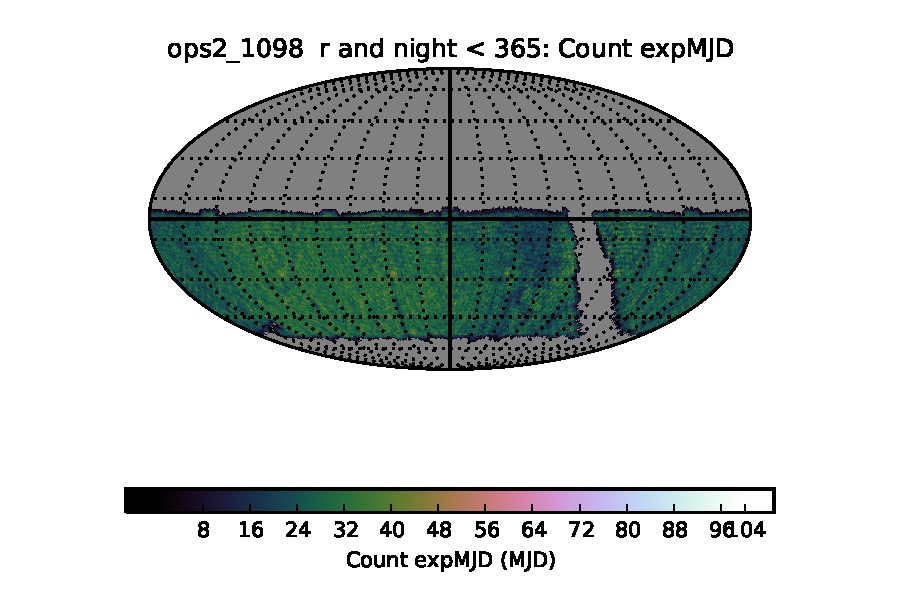
\includegraphics[width=2.3in]{figs/ops2_1098_Count_expMJD_r_and_night_lt_365_HEAL_SkyMap.pdf}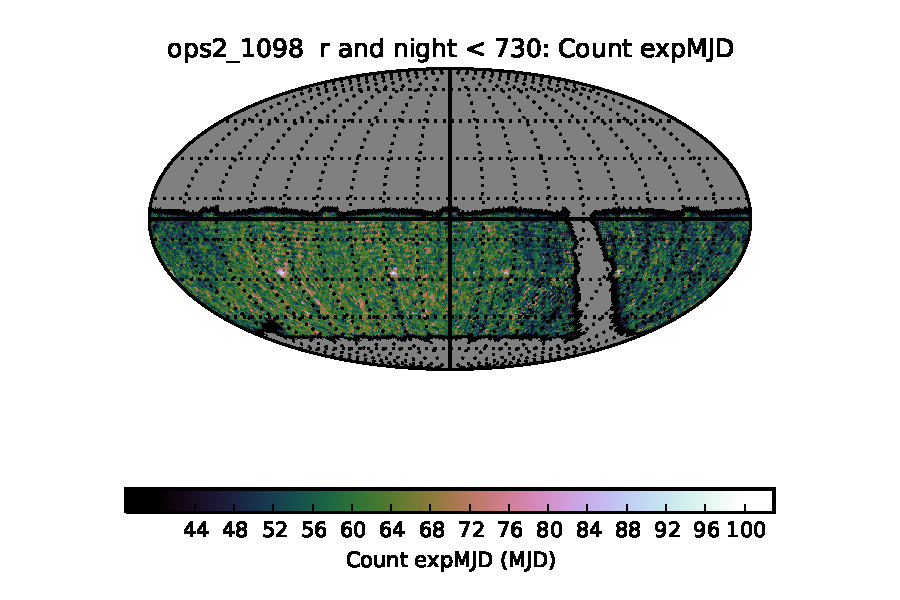
\includegraphics[width=2.3in]{figs/ops2_1098_Count_expMJD_r_and_night_lt_730_HEAL_SkyMap.pdf}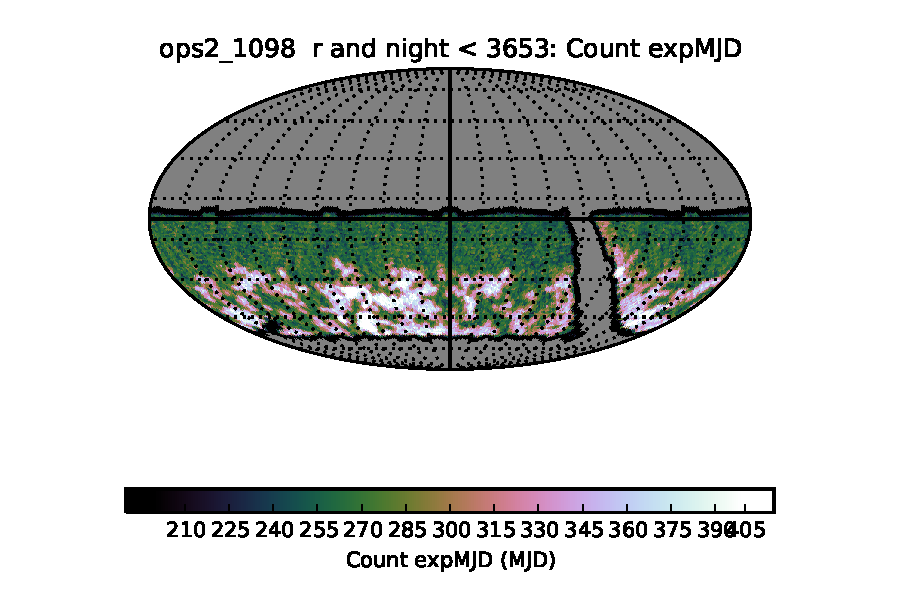
\includegraphics[width=2.3in]{figs/ops2_1098_Count_expMJD_r_and_night_lt_3653_HEAL_SkyMap.pdf} \\
  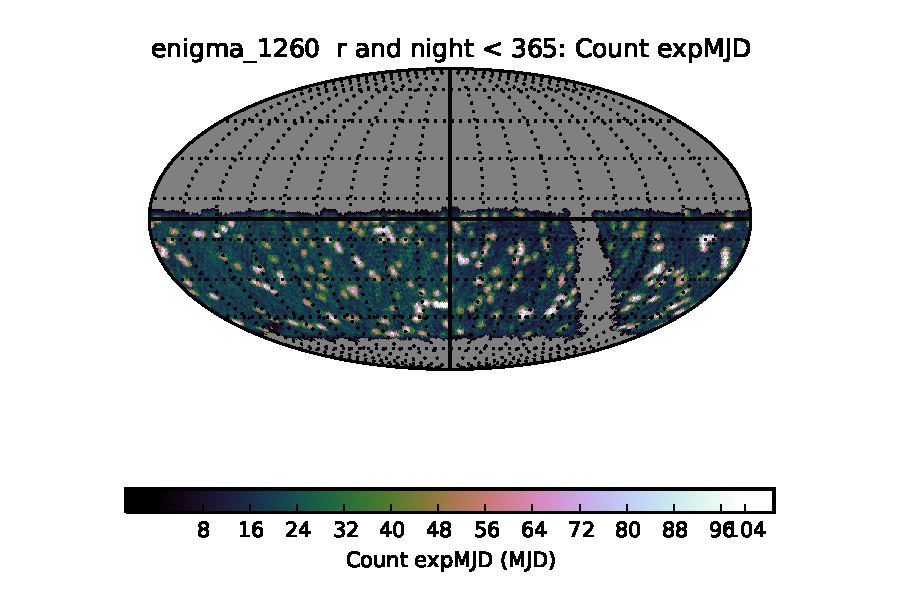
\includegraphics[width=2.3in]{figs/enigma_1260_Count_expMJD_r_and_night_lt_365_HEAL_SkyMap.pdf}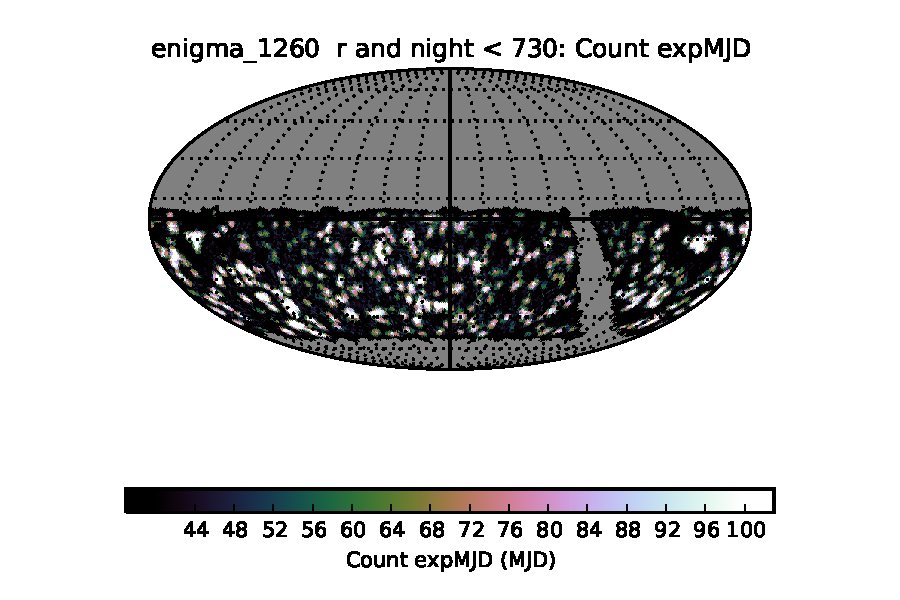
\includegraphics[width=2.3in]{figs/enigma_1260_Count_expMJD_r_and_night_lt_730_HEAL_SkyMap.pdf}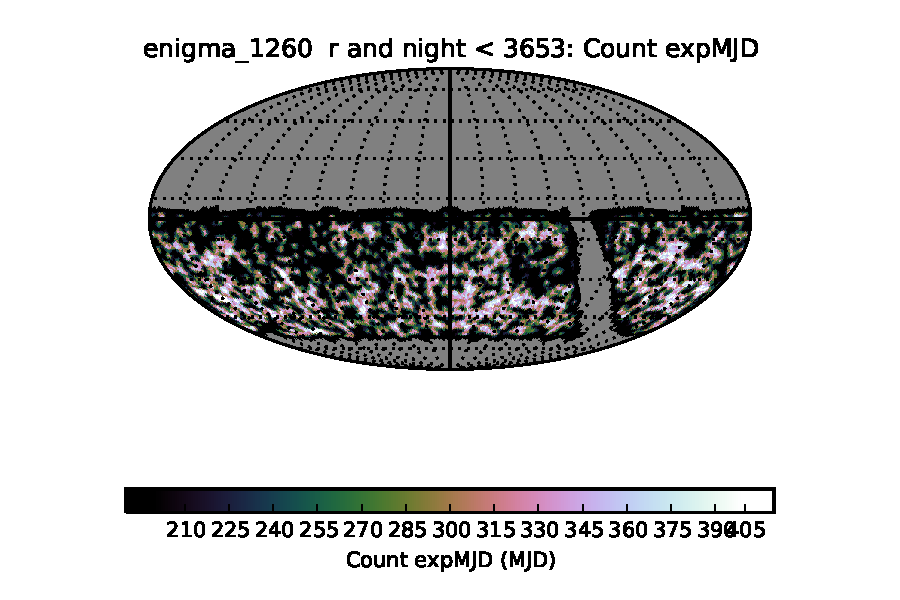
\includegraphics[width=2.3in]{figs/enigma_1260_Count_expMJD_r_and_night_lt_3653_HEAL_SkyMap.pdf}
  \caption{Example of a regular uniform survey (top) and a rolling cadence survey (bottom) after 1, 2, and 10 years in the $r$ filter.  For the regular survey, the number of visits for any part of the sky is relatively constant throughout the survey.  For the rolling cadence simulation, there are regions with many more exposures in year one which then fade in year two as other parts of the sky are emphasized.\label{fig:rollingcadence}}
\end{figure}

% --------------------------------------------------------------------
% --------------------------------------------------------------------
\subsection{Supernovae and Rolling Cadence}
\label{sec:rolling:supernovae}

\noindent{\it Author Name(s)} % (Writing team)

Supernovae as a science topic are addressed elsewhere.
In this section, the demands of SN are used to directly constrain or
orient the rolling cadence development.

Pending more quantitative guidance, the SN objective for rolling cadence is to obtain multicolor time series significantly longer than the typical SN duration, with a cadence significantly faster than uniform.  As an example we discuss the option of a rolling cadence with the regular distribution of filters.

As a simple example, consider improving the cadence by a factor of 2 or 3.  Is we accept that some regions of the sky will be enhanced every year, and that uniform sky coverage will only arrive at the end of 10 years, then we could use, e.g., 10\% of the total epochs in a single roll.  If the enhancement is 2$\times$, each roll would last for $\simeq$ 6 months, with high efficiency for capture of complete SN events.  If the enhancement is 4$\times$, each roll would last for 2 months, with lower efficiency.

If it is important to achieve survey uniformity after 3 years, the available visits for each roll would be reduced also.  With a 2$\times$ enhancement of epoch frequency, a roll would last 2 months.

Some leverage would be gained by using more than 10\% of the available visits for a single roll.  However, this begins to impact the sampling of slow variables reduce schedule flexibility and robustness, and should be approached with caution.

From these examples, it appears that a 2$\times$ enhancement with uniformity closure after 10 years is relatively feasible and promising.  Much higher gains, or more rapid closure, require additional compromises.

% --------------------------------------------------------------------

\subsection{Fast Transients and Rolling Cadence}
\label{sec:rolling:transients}

\noindent{\it Author Name(s)} % (Writing team)

Fast transients as a science topic are addressed elsewhere. In this section, the demands of fast transients are used to directly constrain or
orient the rolling cadence development.

By ``fast transients'', we are referring to events that are sufficiently fast that they are not addressed by the rolling cadence designed for SN observations, and slow enough that they are not covered in ``deep drilling'' type mini-surveys.  For higher tempo rolls, it is quite difficult to obtain full color data, because of the constraints on filter selection.  For this example, we will examine a rolling cadence utilizing only the {\it r} and {\it i} filters, as they are used for most visits. They are close in wavelength, and we assume that sufficient color information will be obtained by the ``background'' uniform survey that continues during a roll.

Again using 10\% of the available visits from the full 10 year survey for a single roll, we find that there would be enough epochs for each roll to acquire 1 visit per day for 21 consecutive days, giving an enhancement of 10$\times$.

Alternatively, the same epochs could be used to observe a target every 20 minutes for 12 hours during a single night (here it is assumed that visit pairs are not required, doubling the available epochs) for an enhancement of 300$\times$.

Several different possible redeployments of portions of a uniform survey have been described, each using 10\% of available time.  Of course it is possible in principal to implement multiple options, sequentially or maybe in parallel in some cases. This may pose considerable challenges to the scheduling strategy design by introducing incompatible boundary conditions.

While rolling cadences are powerful, they have limitations.  For example, sampling events that last longer than $\simeq$1 day and less than $\simeq$ 1 week have the obvious problem of diurnal availability.  In this example, intermediate cadences could be implemented in the circumpolar region, where diurnal access is much extended.  This is an example of a case in which a mini-survey of a limited number of regions could be considered as an alternative to a rolling cadence applied to the entire main survey.

% --------------------------------------------------------------------

\subsection{Constraints, Trades and Compromises for Rolling Cadences}
\label{sec:rolling:trades}

While rolling cadences offer some attractive benefits, it is important to realize that rolling cadences are very highly constrained, and that they do bring disadvantages and compromises.

There are strong arguments against beginning a rolling cadence in the first, or even the second year of the survey.  Early in the survey, it is important to obtain for each field/filter combination, an adequate number of good quality photometric images, and at least one image in excellent seeing, to support closure of photometry reductions and to support generation of template images.

Since major science goals require a significant degree of survey homogeneity,
it may be advisable to implement a strategy that brings the survey to nominal
uniform depth at several times, e.g.\ after 3 or 5 years.  This would strongly
constrain rolling cadences.

Some science objectives favor certain distributions of visits.  For astrometry, visits early and late in the survey and at large parallax factors, are beneficial.  Slow variables may benefit from uniform spacing.  Rolling cadences might impact these constraints either favorably or unfavorably.

Many objectives are served by randomization of observing conditions for each field.  Some rolling cadences could tend to reduce this randomization, for example by acquiring a large number of observations during a meteorologically favorable or unfavorable season, or during a period of instrument performance variance.

Dithering does not work gracefully with a rolling cadence, reducing temporal coverage at the boundaries of the selected sky region.  This is negligible for small dithers, but important for large dithers, which are under consideration.

These cautions illustrate that evaluation of rolling cadences must be based on the full range of schedule performance metrics, and not just those targeted by rolling cadence development.

\subsection{Directions for Future Work with Rolling Cadences}
\label{sec:rolling:directions}

While preliminary experiments with rolling cadences have been carried out with OpSim, these experiments have significant deficiencies, and are not suited for in-depth study as of this writing.  Progress in rolling cadence simulations is expected no sooner than mid to late-2016. Preparatory to that, analysis of cadences described above can guide development of objectives for enhancement by rolling cadence.  

Rolling cadences will be required to pass the same metrics as an other, and general requirements such as sky area, depth and visit count must be met.  Of particular interest will be metrics that clearly distinguish the gains available with rolling cadences - that is, metrics that measure schedule performance for variable targets, and especially those with strong sampling requirements, or more rapid variability.

The following metrics, based on similar metrics developed for particular science objectives, may be useful in tuning rolling cadence performance. 

\begin{enumerate}
\item Observation Pairs histograms.  Visit pairs are simple and easy to quantify.  A pair of visits in the same filter describe a brightness change and constrain the rate of change. A visit pair in different filters (probably not coeval) constrain a color.  These metrics will describe how rapidly LSST can detect a change in the source fluxes. They will be useful for such science as early discovery of SNe, and identification of interesting galactic microlensing events.

\item Observation Triplets histograms. Similar to Pairs, but with closely spaced triplets allowing detection and confirmation of transient events (as described in http://arxiv.org/pdf/1508.03175v2.pdf).

\item Period determination metric.  Compute a measure of the period determination accuracy after a given time interval, as a function of period. A complete analysis would allow use of real light curves for various object types with realistic brightness distributions.  A simpler approach would use a single example light curve and a fixed measurement error value. A simplest approach would be based on the sampling function and its power spectrum (as described in http://arxiv.org/pdf/1508.03175v2.pdf).  This metric group would rate simulation performance for period determination of periodic variables - mostly stars.

\item Sampling of SNe light curves.  The most complete metric would count the number of SNe (of various types) light curves that would be well sampled (according to defined criteria), based on analysis of realistic simulated data.  A simpler metric would be based on estimated sampling requirements and cadence without considering brightness. The latter could be used initially, pending replacement (or calibration) with more extensive simulations.

\item Time series count. For any transient or irregular variable, the optimum observational data will require multiple time and color samples within the duration of the event. Since the category of transients may include discoveries, it is not possible to exhaustively specify the source characteristics. A time series can be defined to consist of a series of samples, over some total duration T, with sampling interval t to tolerance d. The count of time series depends on the total duration, the number of samples, as well as the filter selection, so the challenge is how to visualize this information, and how to extract useful characteristic summary measures of performance.  This type of data can be valuable for identification and study of rapid phenomena such as stellar flares, binary mass transfer events, and exoplanet transits, and for slower events such as AGN reverberation mapping.

\end{enumerate}

% ====================================================================

\navigationbar

% ====================================================================
% commands for stand-alone printing
% \bibliographystyle{apj}
% \bibliography{references}
% \end{document}
% ====================================================================
